\chapter{Introduction}
\label{cha:intro}
Battery electric vehicles are becoming a fundamental part of the transportation industry. This technology shift brings new challenges in many fields of study. This thesis overviews some of these challenges regarding battery management systems on electric cars.\\
Batteries are complex electro-chemical components that need to be constantly monitored in order to ensure maximum safety and efficiency. Especially in the automotive domain, where vehicles are often subject to unoptimal and variable working conditions, a system that ensures the correct operation of the battery is necessary. Since the BMS can influence the performance of a vehicle, it is important to have a well designed and calibrated management system that isn't too invasive to the vehichle's operation, but retains acceptable levels of safety.

\section{Formula SAE}
Formula SAE is an international design competition founded by the Society of Automotive Engineers in 1980, in which university students have to develop, build and race an open-wheel, single seater race car.\\
In Europe, Formula Student Germany releases the rulebook \cite{fsg2020} that specifies how a Formula SAE car must be constructed in order to participate in european competitions.\\
The following sections summarize how the powertrain is architectured.
\section{Tractive System}
\begin{figure}[h]
    \centering
    \ctikzset{bipoles/crossing/size=.6}
\begin{circuitikz} \draw
    (0,1) to[battery=\(BAT\)] ++(0,3)

    (0,4) to[nos=\(AIR-\), n=airm] ++(5,0)
    to (5, 2.6) -- ++(2,0) -- (7, 4.5) -- ++(1.5,0)
    (7, 2.4) -- (7.75,2.4) -- (7.75,3.5) -- (8.5,3.5)
    (8.5,4.5) to[C=\(C_1\)] (8.5,3.5)

    (0,1) to[nos=\(AIR+\), n=airp] ++(5,0)
    to (5,2.4) -- ++(2,0) -- (7, 0.5) -- ++(1.5,0)
    (7, 2.6) to[crossing] ++(1.5,0) -- (8.5,1.5)
    (8.5,1.5) to[C=\(C_2\)] (8.5,0.5)

    (0.5,1) -- ++(0,-1)
    to[nos=\(S_p\),n=pre_sw] ++(2, 0)
    to[R=\(R_p\),n=pre_sw] ++(2,0)
    to ++ (0,+1)

    (8.5,0.5) edge[dashed] ++(1,0)
    (8.5,1.5) edge[dashed] ++(1,0)

    (8.5,3.5) edge[dashed] ++(1,0)
    (8.5,4.5) edge[dashed] ++(1,0)

    {[anchor=north] (6,2.4) node {\(Bus_+\)} [anchor=south] (6,2.6) node {\(Bus_-\)}};

    \draw (11.5,3.75) node[elmech](M1){M1}
    (9.75,4.9) -- ++(1,0) -/ (M1.150)
    (9.75,3.75) -| (M1.180)
    (9.75,2.65) -- ++(1,0) -/ (M1.210)
    ;
    \draw (11.5,1.25) node[elmech](M2){M2}
    (9.75,2.35) -- ++(1,0) -/ (M2.150)
    (9.75,1.25) -| (M2.180)
    (9.75,0.1) -- ++(1,0) -/ (M2.210)
    ;

    \draw[dotted] (-2,5) rectangle (5.25,-0.5) node[at start, right, fill=white] {Pack};
    \draw[dashed] (6.75,5) rectangle (9.75,2.55) node[at start, right, fill=white] {Inverter 1};
    \draw[dashed] (6.75,0) rectangle (9.75,2.45) node[at start, right, fill=white] {Inverter 2};
\end{circuitikz}
    \caption{Tractive system block schema}
    \label{fig:tractive_system}
\end{figure}
The tractive system is the whole high-voltage system of the car. It comprises the battery pack, the inverters and the electric motors that drive the wheels of the car.
E-Agle TRT's car is powered by two independent three-phase permanent-magnet motors that drive the rear axle. Each motor is controlled by a motor controller that converts the direct current from the battery into three-phase alternating current for the motor. By varying the current's frequency and intensity, the controllers are able to define the motor's speed and torque.

\section{Battery Architecture}
A battery is an electrical energy storage system that relies on chemical reactions to generate a voltage. The main properties of a battery are: nominal voltage, internal resistance, energy capacity and maximum discharge rate.\\
The voltage of a battery is influenced by many factors including: state of charge, temperature and applied load.\ The open-circuit voltage of a Lithium-Ion battery cell is 4.2V at 100\% state of charge and 3.0V at 0\%. The rules \cite[EV 5.8.6]{fsg2020} state that this voltage range can only be exceeded for 500ms, after which the battery pack must shut down, cutting power to the rest of the tractive system. It is the duty of the BMS to ensure the compliance to this rule.\\
When a load is applied to a cell, the voltage drops according to Ohm's law: $V_{dropped} = R_{internal}*I_{load}$. The higher the current drawn, the higher the voltage drop. In high power applications, this phenomenon can significantly reduces the usable energy storage of the battery.

\subsection{Battery Pack}
A battery pack is a group of cells connected in series and parallel to form a bigger battery. Arranging the cells in series means that the current will only travel down a single path, passing through every cell. In this case the voltage of the pack is equals to the sum of each series.\\
In a parallel arrangement, electrons travel down multiple paths, splitting the current across more cells. This increases the current output of the battery, but the total voltage is the same of a single cell's.\ A parallel connection is also called a module.
\begin{figure}[H]
    \centering
    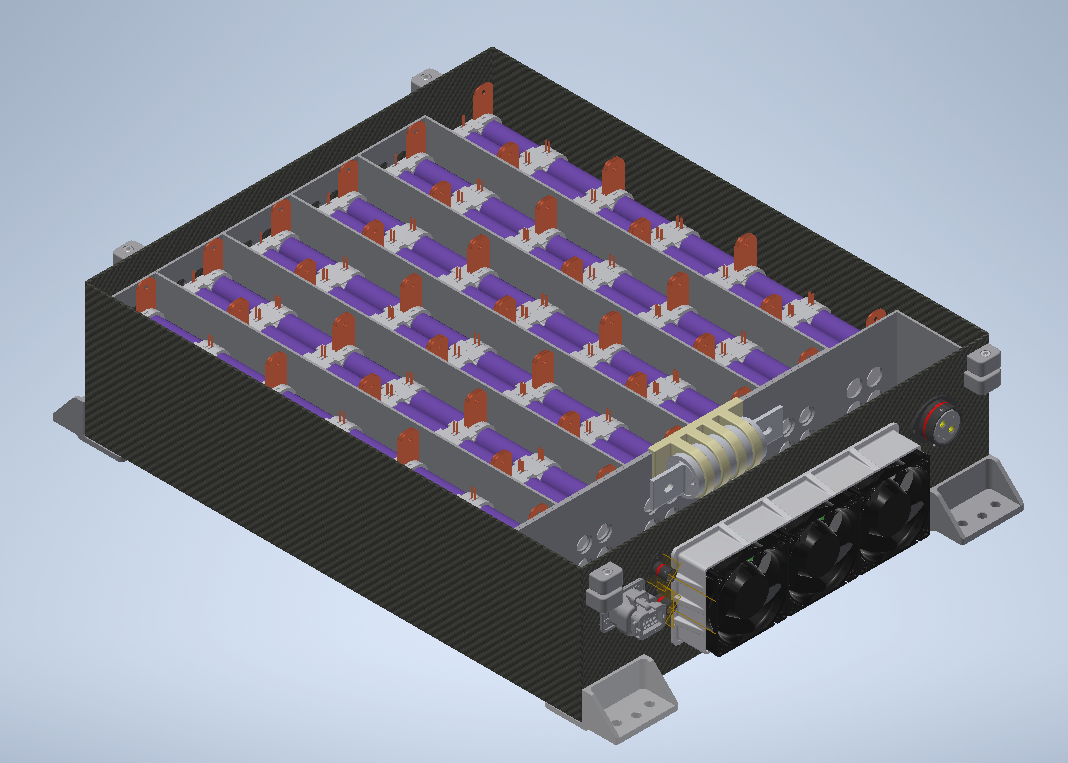
\includegraphics[scale=0.5]{pictures/pack.png}
    \caption{3D model of Fenice's battery pack}
    \label{fig:pack}
\end{figure}
The structure of a battery pack is decided considering its specific application. For example, in an high power context, higher voltage batteries are more desirable because for the same power, less current is required, decreasing heat losses in cables and conductors. If higher current is requested, more cells in parallel could be arranged, increasing the total energy storage and weight as a consequence.

In a Formula SAE car, the optimal setup is a lightweight, high-voltage and high-power battery pack. The rulebook limits voltage to 600V \cite[EV 4.1.1]{fsg2020} and power to 80kW \cite[EV 2.2.1]{fsg2020}, so the resulting battery will have as many cells in series as permitted and as few parallels as needed to reach the required power and capacity target. E-Agle TRT car's battery features 108 cells in series and only 4 in parallel, for a total of 432 cells and a nominal voltage of 388.8V (3.6V per cell). The high power requirement is fullfilled by the use of high-discharge rate cells, 45A in this case, that result in an output of 180A of continuous discharge current. As a consequence, The maximum theoretical power output is \~{}70kW and the energy capacity amounts to 6.2kWh.

As explained in figure \ref{fig:naming}, the pack is subdivided in physical blocks that can be summarised as follows:
\begin{figure}[h]
    \centering
    \begin{circuitikz}
    % Cell
    \draw (0,2) to[battery1] (0,3);
    \draw node[circle,draw,anchor=center,scale=4,label=Cell] (cell) at (0,2.5) {};

    % Cell to Module
    \draw node[circle,draw,anchor=center,scale=2.5] (ctm) at(2.25,2.5) {};
    \draw[->] (cell.east) -- (ctm.west);

    % Module
    \draw (2.75,1.5) -- ++(0,0.5) -| ++(-0.5,0) to[battery1] ++(0,1) -| ++(0.5,0.5)
    (2.75,2) -- ++(0.5,0) to[battery1] ++(0,1) -- ++(-0.5,0);
    \draw (3.25,2) edge[dotted] ++(0.5,0)
    (3.25,3) edge[dotted] ++(0.5,0);
    \draw node[circle,draw,anchor=center,scale=7,label=Module] (module) at (2.75,2.5) {};

    % Module to Block
    \draw node[circle,draw,anchor=center,scale=2.5] (mtb) at(6.5,2.5) {};
    \draw[->] (module.east) -- (mtb.west);

    % Block
    \draw (6.5,1) to[battery1] ++(0,1) to[battery1] ++(0,1) to[battery1] ++(0,1);
    \draw node[circle,draw,anchor=center,scale=9,label=Block] (block) at (6.5,2.5) {};

    % Block to Segment
    \draw[->] (block.east) -- (9.65,2.5);

    % Segment
    \draw (9.625,3) -- ++(0,+0.25);
    % 1
    \draw[solid] (9.5,2) rectangle ++(0.25,1);
    \draw (9.625,2) -- ++(0,-0.25) -| ++(0.5,0.25) ;
    % 2
    \draw[solid] (10,2) rectangle ++(0.25,1);
    \draw (10.125,3) -- ++(0,0.25) -| ++(0.5,-0.25) ;
    % 3
    \draw[solid] (10.5,2) rectangle ++(0.25,1);
    \draw (10.625,2) -- ++(0,-0.25) -| ++(0.5,0.25) ;
    % 4
    \draw[solid] (11,2) rectangle ++(0.25,1);
    \draw (11.125,3) -- ++(0,0.25) -| ++(0.5,-0.25) ;
    % 5
    \draw[solid] (11.5,2) rectangle ++(0.25,1);
    \draw (11.625,2) -- ++(0,-0.25) -| ++(0.5,0.25) ;
    % 6
    \draw[solid] (12,2) rectangle ++(0.25,1);
    \draw (12.125,3) -- ++(0,0.25);

    \draw node[circle,draw,anchor=center,scale=10,label=Segment] (segment) at (10.825,2.5) {};

    % Segment to Pack
    \draw[->] (segment.east) -- (14.15,2.5);

    % Pack
    \draw (14.125,3) -- ++(0,+0.25);
    % 1
    \draw[solid] (14,2) rectangle ++(0.25,1);
    \draw (14.125,2) -- ++(0,-0.25) -| ++(0.5,0.25) ;
    % 2
    \draw[solid] (14.5,2) rectangle ++(0.25,1);
    \draw (14.625,3) -- ++(0,0.25) -| ++(0.5,-0.25) ;
    % 3
    \draw[solid] (15,2) rectangle ++(0.25,1);
    \draw (15.125,2) -- ++(0,-0.25) -| ++(0.5,0.25) ;
    % 4
    \draw[solid] (15.5,2) rectangle ++(0.25,1);
    \draw (15.625,3) -- ++(0,0.25) -| ++(0.5,-0.25) ;
    % 5
    \draw[solid] (16,2) rectangle ++(0.25,1);
    \draw (16.125,2) -- ++(0,-0.25) -| ++(0.5,0.25) ;
    % 6
    \draw[solid] (16.5,2) rectangle ++(0.25,1);
    \draw (16.625,3) -- ++(0,0.25);

    \draw node[circle,draw,anchor=center,scale=10,label=Pack] (pack) at (15.4,2.5) {};

\end{circuitikz}
    \caption{Battery pack elements naming scheme}
    \label{fig:naming}
\end{figure}

\begin{itemize}
    \item A cell is a single battery.
    \item A parallel of four cells forms a module (also called cell, since the voltage is the same).
    \item Blocks are a series of three modules, that are mounted in a single independent element.
    \item The rulebook requires the separation of the pack into segments with precise physical and electrical characteristics \cite[EV 5.3.2]{fsg2020}. In this case a segment is a series of six blocks, totalling a maximum voltage of 75.6V ($4.2V*3\ modules*6\ blocks$) and \~1.2kWh of energy, below the limit of 120V and 1.6 kWh mandated by the rules.
    \item Finally, the battery pack is a collection of six segments connected in series.
\end{itemize}

\subsection{Internal Connections}
To better control the pack, two Accumulator Isolation Relays (AIR) \cite[EV 5.6]{fsg2020} are located at both poles of the pack to disconnect its output when not needed. These relays are controlled by the BMS and can also be switched off by external devices such as emergency buttons and sensors located around the car.
\begin{figure}[h]
    \centering
    \ctikzset{bipoles/crossing/size=.6}
\begin{circuitikz} \draw
    (0,1) to[battery=\(BAT\),american] ++(0,3)

    %% Negative battery bus
    (0,4) to[fuse=\(F\)] ++(1.5,0) to[nos=\(AIR-\), n=airm] ++(2,0) -- ++(1.5,0)
    -- (5, 2.6) to[short, -*] ++(2,0) -- (7, 4.5) -- ++(1.5,0)

    %% Inverter 1
    (7, 2.4) to[short, *-] (7.75,2.4) -- (7.75,3.5) -- (8.5,3.5)
    (8.5,3.5) to[C=\(C_1\), n=c1, *-*] (8.5,4.5)

    (8.5,0.5) -- ++(0.75,0)
    (8.5,1.5) -- ++(0.75,0);
    \draw[solid] (9.25,3.25) rectangle ++(0.5,1.5);
    \path (9.25,3.25) -- ++(0,-0.5);
    \draw[dotted] (7.3,5) rectangle (10,3) node[at start, right, fill=white] {Inverter 1};

    %% Positive battery bus
    \draw (0,1) to[nos=\(AIR+\), n=airp] ++(5,0)
    to (5,2.4) -- ++(2,0) -- (7, 0.5) -- ++(1.5,0)

    %% Inverter 2
    (7, 2.6) to[crossing] ++(1.5,0) -- (8.5,1.5)
    (8.5,0.5) to[C=\(C_2\), *-*] (8.5,1.5)

    (8.5,3.5) -- ++(0.75,0)
    (8.5,4.5) -- ++(0.75,0);
    \draw[solid] (9.25,1.75) rectangle ++(0.5,-1.5);
    \draw[dotted] (7.3,0) rectangle (10,2) node[at start, right, fill=white] {Inverter 2};

    %% Pre-charge circuit
    \draw (0.5,1) to[short, *-] ++(0,-1)
    to[nos=\(S_p\),n=pre_sw] ++(2, 0)
    to[R=\(R_p\),n=pre_sw] ++(2,0)
    to[short, -*] ++(0,+1)

    {[anchor=north] (6,2.4) node {\(Bus_+\)} [anchor=south] (6,2.6) node {\(Bus_-\)}};

    %% Motor 1
    \draw (11,4) node[elmech](M1){M1}
    (9.75,4.65) -- ++(0.75,0) -- (M1.150)
    (9.75,4) -| (M1.180)
    (9.75,3.35) -- ++(0.75,0) -- (M1.210)
    ;

    %% Motor 2
    \draw (11,1) node[elmech](M2){M2}
    (9.75,1.65) -- ++(0.75,0) -/ (M2.150)
    (9.75,1) -| (M2.180)
    (9.75,0.35) -- ++(0.75,0) -/ (M2.210)
    ;

    \draw[dotted] (-2,5) rectangle (5.25,-0.5) node[at start, right, fill=white] {Battery Pack};


\end{circuitikz}
    \caption{Tractive system schema}
    \label{fig:tractive_system_detail}
\end{figure}

\section{Battery Management}
Battery management is a collection of operations that ensure the safety and efficiency of the battery pack's functioning.\\
A battery management system should constantly measure cell temperatures and voltages along with the total pack current output and check that each of those values is within specification. If anomalies are detected, the battery should be disconnected immediately.\\
Advanced BMS solutions communicate their state of operation with other devices, and turn the battery on or off following external signals.\\
Moreover, during battery charging, the BMS should handle the current delivery of the charger, to maximize charging speed while keeping high safety levels.\\
As the BMS manages a critical piece of hardware, its software must adhere to strict coding standards and should be tested thoroughly, to avoid potentially catastrophic failures.

\subsection{Module Balancing}
Cells are not perfectly identical and can have slight variations in internal resistance between each other. These differences mean that after some use, modules can start to deviate in voltage between one another. If a battery has an higher voltage than average, the pack can only be charged to the voltage of said cell, while the remaining batteries are not fully charged. The same applies during discharge: if a cell is more discharged than the others, it constraints the maximum depth of discharge to the lower-voltage cell.
This issue limits the maximum energy storage available for use. The solution involves charging or discharging every module until they all are within acceptable tolerance.\\

